%

\documentclass[aspectratio=169]{beamer}

\usepackage{tikz}
\usepackage{xspace}
\usepackage{graphicx}
\usepackage{etoolbox}
\usepackage{calc}

\usetikzlibrary{decorations.pathreplacing,decorations.markings,snakes}
\usetikzlibrary{shapes.symbols}

\setbeamercovered{invisible}
\usenavigationsymbolstemplate{}

%\newcommand\step[1]{\textit{Step #1.}}
\newcommand\step[1]{\tikz[anchor=base, baseline]{\node [draw, circle, inner sep=0pt, minimum width=13pt, fill=black!10] at (0,0) {#1};}}

\newlength\pw
\setlength\pw{16cm}
\newlength\rw
\newlength\lw
\newcommand\splitpage[3]{
\begin{minipage}{#1\pw}
    \raggedright #2
\end{minipage}
\setlength\lw{#1\pw}
\setlength\rw{13cm-\lw}
\begin{minipage}{\rw}
    \raggedright #3
\end{minipage}
}
\def\gap{5pt}
\def\vgap{\vspace{\gap}}

\makeatletter
\setbeamertemplate{footline}
{
  \leavevmode%
  \hbox{%
  \begin{beamercolorbox}[wd=\paperwidth,ht=0ex,dp=1ex,right]{date in head/foot}%
    \large\insertframenumber\hspace*{1ex} 
  \end{beamercolorbox}}%
  \vskip3pt%
}
\makeatother

\newcommand\picturefamily[1]{\ensuremath{\begin{tikzpicture}[outer sep=0pt,inner sep=0pt]#1\end{tikzpicture}}}

\tikzset{string/.style={line width=0.7pt}}
\tikzset{button/.style={draw, line width=0.7pt, minimum height=0.6cm, minimum width=0.6cm, inner sep=0pt}}
\tikzset{M/.style={button, fill=red!70}}
\definecolor{myblue}{rgb}{0.1,0.5,1}
\tikzset{H/.style={button, fill=myblue}}
\tikzset{P/.style={button, fill=black,text=white}}
\tikzset{Z/.style={button, fill=green!95!black}}
\tikzset{miniCZ/.style={button, fill=white}}
\tikzset{CZ/.style args={#1}{button, fill=white, minimum height=#1cm+0.6cm }}
\tikzset{result/.style={red, above=0.24cm}}
\newcommand\inlinebutton[2]{\ensuremath{\smash{\begin{aligned}\tikz{\node [#1] {#2};}\end{aligned}}}\xspace}
\newcommand\fullheightbutton[2]{\ensuremath{{\begin{aligned}\tikz{\node [#1] {#2};}\end{aligned}}}\xspace}
\newcommand\inlineM{\inlinebutton{M}{M}}
\newcommand\inlineH{\inlinebutton{H}{H}}
\newcommand\inlineP{\inlinebutton{P}{P}}
\newcommand\inlineZ{\inlinebutton{Z}{Z}}
\newcommand\inlineCZ{\inlinebutton{button, fill=white}{CZ}}
\newcommand\fullheightM{\fullheightbutton{M}{M}}
\newcommand\fullheightH{\fullheightbutton{H}{H}}
\newcommand\fullheightP{\fullheightbutton{P}{P}}
\newcommand\fullheightZ{\fullheightbutton{Z}{Z}}
\newcommand\fullheightCZ{\fullheightbutton{button, fill=white}{CZ}}

\newcommand\ignore[1]{}
\setbeamertemplate{itemize item}{\raise0pt\hbox{\donotcoloroutermaths\color{black}$\bullet$}}
\begin{document}

{
\setbeamertemplate{footline}{} % Prevent title slide having a number
\begin{frame}
\vspace{-20pt}
\[
\hspace{-2cm}

\begin{tikzpicture}[xscale=1.2, yscale=1.8]
\foreach \x/\y in {0/red,1/orange,2/yellow,3/green,4/blue} {
  \path [fill=\y] (0,\x) rectangle +(\textwidth,1);
}
\path [use as bounding box] (current bounding box.south west) rectangle (current bounding box.north east);
\node [scale=2.5, white, yscale=3.04] at (0.5*\textwidth,2.29) {\Huge\bf a       QUBIT.ZONE};
\end{tikzpicture}
\hspace{-2cm}
\]

\end{frame}
}

% Make subsequent slides start from 1
\addtocounter{framenumber}{-1}

\usebackgroundtemplate{$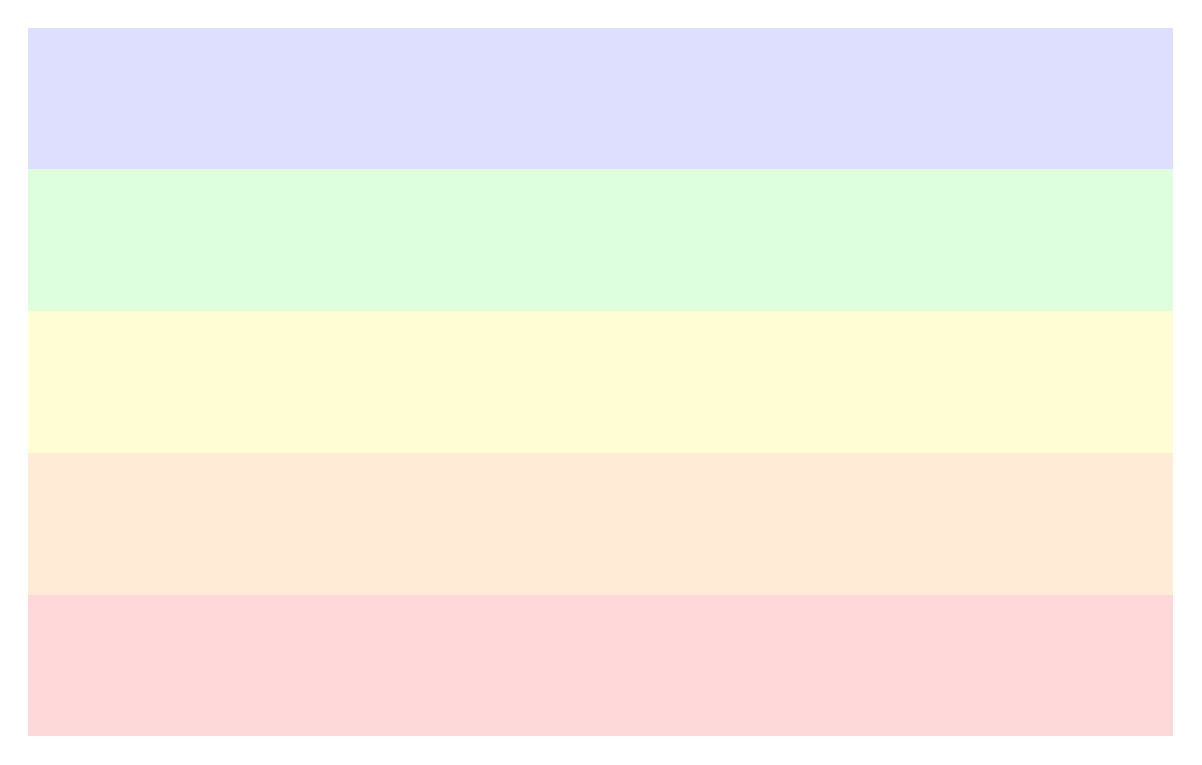
\begin{tikzpicture}[xscale=1.2, yscale=1.8]
\foreach \x/\y/\z in {0/red/15,1/orange/16,2/yellow/17,3/green/13,4/blue/13} {
  \path [fill=\y!\z] (0,\x) rectangle +(\textwidth,1);
}
\end{tikzpicture}$}


\setbeamertemplate{frametitle}{\color{black}\centering\Huge\bfseries\insertframetitle\par\vskip-6pt}

\begin{frame}
\frametitle{QUANTUM COMPUTERS}


\splitpage{0.4}{
\uncover<1->{Scientists around the world are racing to build the first \textit{quantum computer}.}

\vspace{0.5cm}
\uncover<2->{These will give our civilization incredible new abilities to:}
\begin{itemize}
\uncover<2->{\item design drugs;}
\uncover<3->{\item analyze data;}
\uncover<4->{\item break encryption;}
\uncover<5->{\item build intelligent robots.}
\end{itemize}

\vspace{0.5cm}
\uncover<7->{But what are the \textit{fundamental ideas} that underlie quantum computers?}
}
{
\picturefamily{
\uncover<1->{\node [anchor=north west] at (0,0) {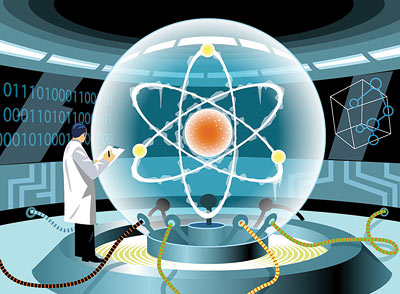
\includegraphics[width=7cm]{images/quantum_atom_in_room}};}
\uncover<2->{\node [anchor=north west] at (-0.5,-0.5) {
\includegraphics[height=3cm]{images/free/drugs}};}
\uncover<3->{\node [anchor=north] at (3.5,-1) {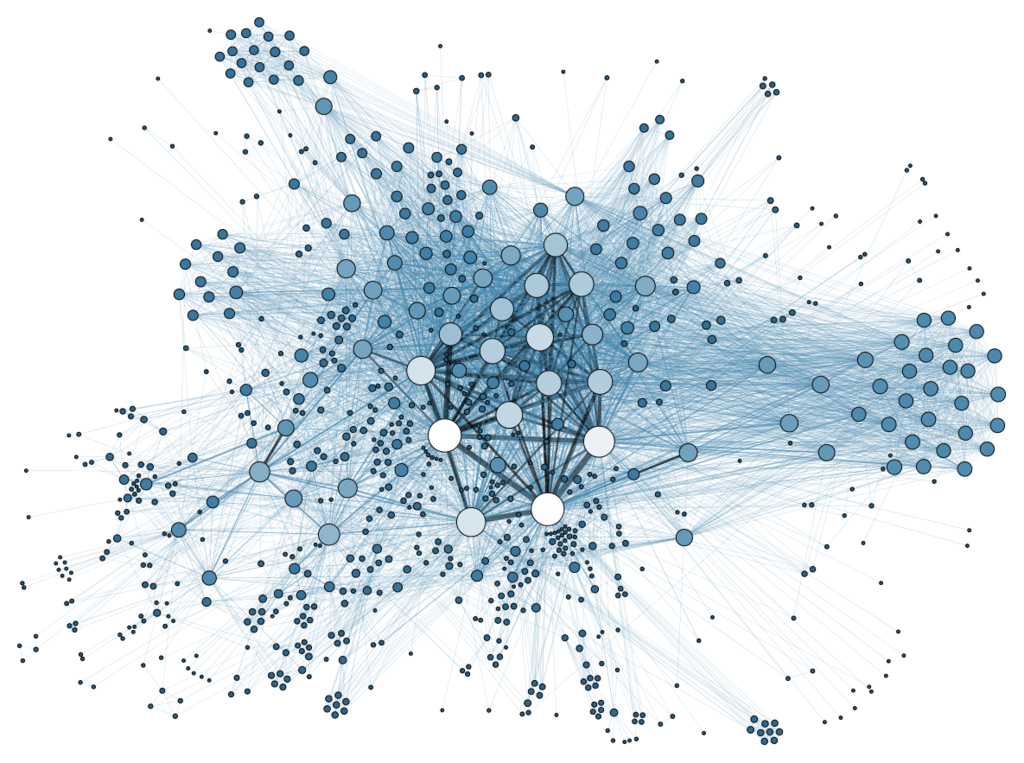
\includegraphics[height=3cm]{images/free/data}};}
\uncover<4->{\node [anchor=north east] at (7.5,-1.5) {
\includegraphics[height=3cm]{images/free/encryption}};}
\uncover<5->{\node [anchor=north west] at (0.5,-2) {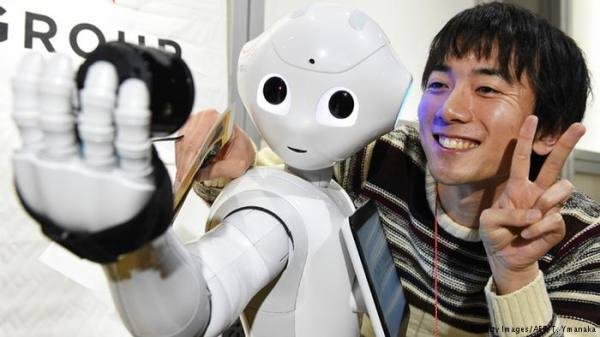
\includegraphics[height=3.5cm]{images/nonfree/friendly_robot}};}
\uncover<6->{\node [anchor=north west] at (1,-2.5) {
\includegraphics[height=4cm]{images/terminator}};}
}}

\end{frame}

\begin{frame}
\frametitle{THE QUANTUM WORLD}

\splitpage{0.51}{
\vspace{5pt}
\uncover<1->{Atoms and electrons are some of the smallest things that exist.}

\vspace{10pt}
\uncover<2->{They obey the laws of \emph{quantum theory}--- mysterious, counterintuitive and surprising.}
}
{
\picturefamily{
\uncover<1->{\node [anchor=north] at (0,0) {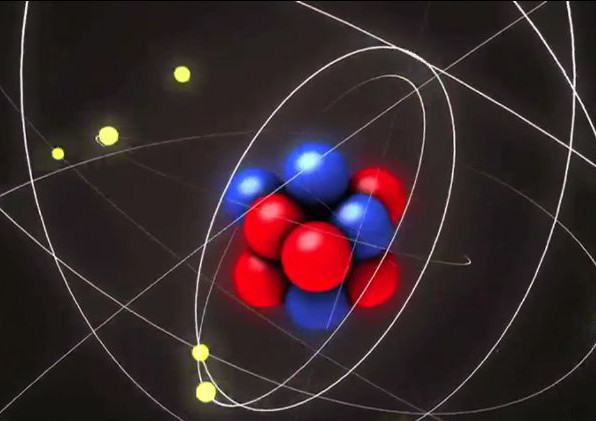
\includegraphics[height=3cm]{images/quantum_particles}};}
}}


\vspace{20pt}

\pause\pause
Quantum objects can do lots of amazing things:
\begin{itemize}
\pause
\item \textit{Superposition}---be in two places at once.

\pause\item \textit{Entanglement}---different objects that behave in exactly the same way.

\pause\item \textit{Teleportation}---jump straight from one place to another.
\end{itemize}

\pause
\vspace{10pt}
Quantum computers will exploit these to perform their amazing tasks.

\end{frame}


\newcommand\col[2]{\begin{minipage}{#1\textwidth}\raggedright #2\end{minipage}}


\begin{frame}
\frametitle{QUBITS}

\def\gap{10pt}
\vspace{15pt}
\col{0.5}{
Ordinary computers are built from \textit{bits}, which can equal 0 or 1.

\vgap
\uncover<2->{
Quantum computers will be built from \textit{qubits}. You've got one in front of you.*}

\vgap
\uncover<3->{It has got lots of mysterious buttons.
\\
Give them a try!}

\vgap
\uncover<4->{
We will use these qubits to investigate the properties of quantum computers.}

\vgap
\uncover<2->{
\scriptsize * Just a \textit{simulated} qubit unfortunately :(.}
}
\col{0.4}{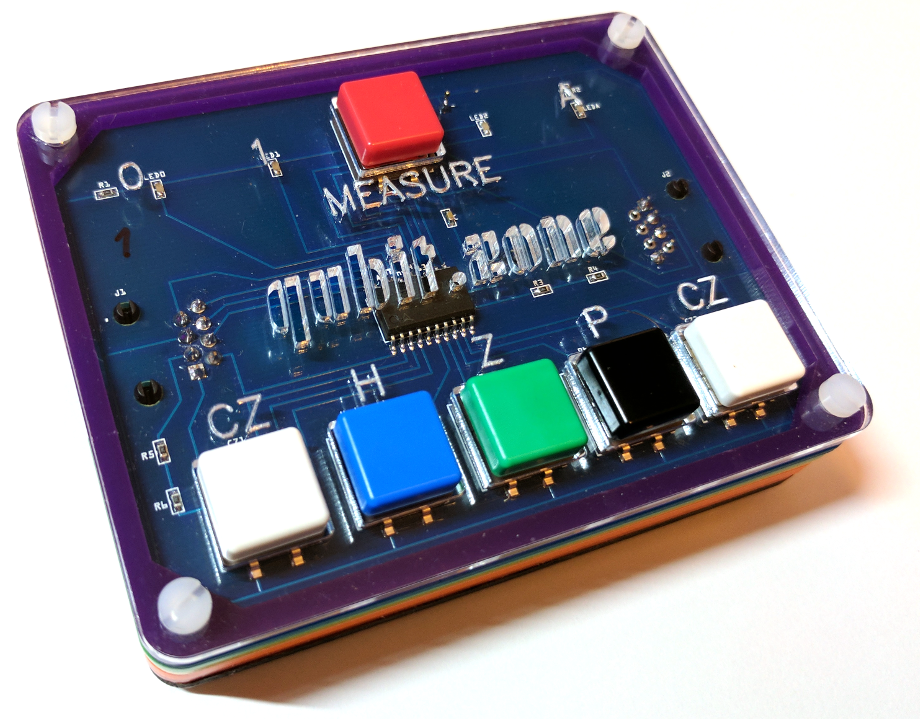
\includegraphics[height=6cm]{images/qubit_1.png}}

\end{frame}

\begin{frame}
\frametitle{QUANTUM PROGRAMS}
\textbf{Let's try it!} Press \inlineH, \inlineZ or \inlineP. A green/yellow LED lights up at the top right corner of your qubit! This shows that the qubit is doing something.
\vspace{10pt}

\vgap Press \inlineM. Now also a red LED lights up! 
\vspace{10pt}


\vgap Press \inlineCZ. Nothing happens. \inlineCZ needs two qubits to work.
\vspace{10pt}

\vgap Get into pairs and connect your qubits with a cable. Now both press \inlineCZ at the connected side of your qubit at the same time. 
\vspace{10pt}
\vgap 

Pressing buttons on many connected qubits in a certain order is called a \textit{quantum program}. You've just built your first quantum program!


\end{frame}
\begin{frame}
\frametitle{SUPERPOSITION}

\vspace{10pt}
\splitpage{0.55}
{
A famous example is Schr\"odinger's Cat.

\def\gap{15pt}
\vgap
\uncover<2->{Simultaneously dead \textit{and} alive ...}

\vgap
\uncover<3->{... but when we look, it's either dead \textit{or} alive.}

\vgap
\uncover<4->{Scientists call this \textit{measurement}.

It destroys the superposition.}
}
{
\picturefamily{
\node at (0,0) {
\includegraphics[height=6cm]{images/schrodingers_cat_wanted}};
}
}
\end{frame}

\def\gap{10pt}

\begin{frame}
\frametitle{SUPERPOSITION}

\textbf{Let's try it!}

\vgap\pause
\textit{Step 1.} Press \inlineM to measure at your qubit. It's  storing 0 or 1.

\vgap\pause
\textit{Step 2.} Press \inlineH to put your qubit into superposition. Now it's storing 0 \textit{and} 1.

\vgap\pause
\textit{Step 3.} Press \inlineM to measure at your qubit. The superposition has collapsed!

\vspace{30pt}
\pause
Sometimes we will need to \textit{force} a qubit to store 0. 

\vgap\pause
Do this by pressing \inlineH then \inlineM repeatedly, until you get 0.

\end{frame}

\ignore{
\begin{frame}
\frametitle{QUANTUM PROGRAMS}
\vspace{25pt}
A \textit{quantum program} is a recipe which tells you which buttons have to be pressed in which order. Here's an example:
\vspace{25pt}
\[ 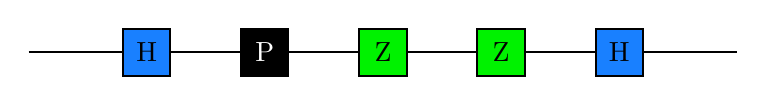
\begin{tikzpicture}[xscale=3]
\draw[string](0,0) to +(3,0);
\node[H] at (0.5,0) {H};
\node[P] at (1,0) {P};
\node[Z] at (1.5,0) {Z};
\node[Z] at (2,0) {Z};
\node[H] at (2.5,0){H};
\end{tikzpicture}
\]

\vspace{10pt}Usually, quantum programs use more than one qubit:
\vspace{10pt}
\[ 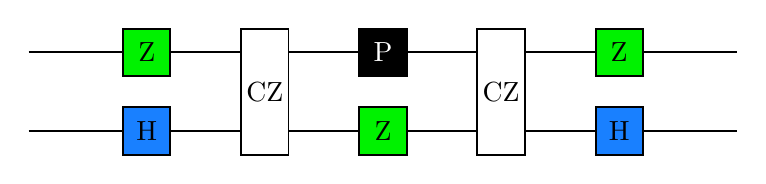
\begin{tikzpicture}[xscale=3]
\draw[string] (0,0) to + (3,0);
\draw[string] (0,1) to + (3,0);
\node[H] at (0.5,0) {H};
\node[Z] at (0.5,1) {Z};
\node[P] at (1.5,1) {P};
\node[Z] at (1.5,0) {Z};
\node[Z] at (2.5,1) {Z};
\node[H] at (2.5,0){H};
\node[CZ={1}] at (2,0.5) {CZ};
\node[CZ={1}] at (1,0.5) {CZ};
\end{tikzpicture}
\]
\end{frame}
}

\begin{frame}
\frametitle{ENTANGLEMENT}

\def\gap{5pt}

\vspace{10pt}

\splitpage{0.5}{
Two quantum systems can sometimes become strongly connected, even if they are far apart.

\vgap\uncover<2->{
This is called \textit{entanglement}.}

\vgap\uncover<3->{
Although individually each system is unpredictable, they will copy each other exactly.}
}{
\raggedright
$\begin{aligned}
\tikz{\node at (0,0) {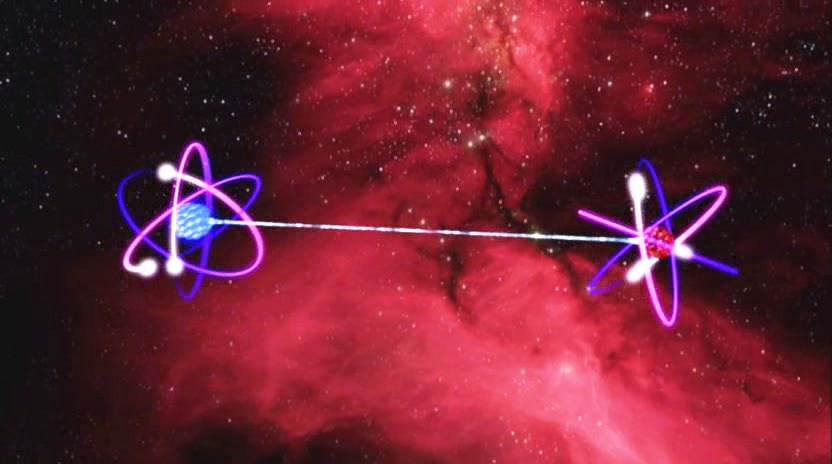
\includegraphics[height=2.7cm]{images/nonfree/entangled}};}
\end{aligned}$
}

\splitpage{0.53}{
\uncover<4->{Einstein hated quantum entanglement.}

\vgap\uncover<5->{He thought it was ``spooky'', and showed that quantum mechanics wasn't a \textit{complete} theory.}

\vgap
\uncover<6->{He was wrong! Silly Einstein.}
}{
\hspace{2cm}
\begin{tikzpicture}
\uncover<4->{\node at (0,0) {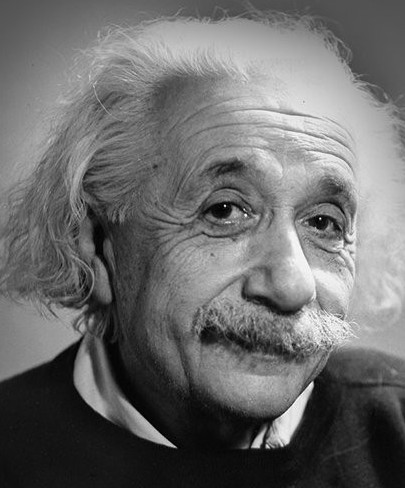
\includegraphics[height=3.5cm]{images/einstein}};}
\uncover<5->{\node at (0.5,-0.25) {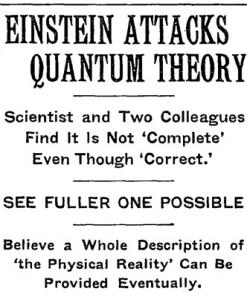
\includegraphics[height=3.5cm]{images/free/nyt_1935}};}
\uncover<6->{\node at (1,-0.5) {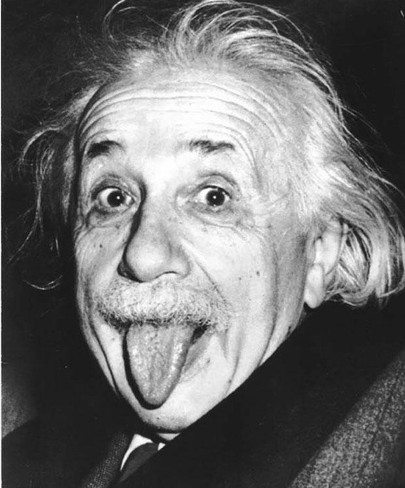
\includegraphics[height=3.5cm]{images/einstein_silly}};}
\end{tikzpicture}
}

\end{frame}

\tikzset{cable/.style={snake}}

\begin{frame}
\frametitle{ENTANGLEMENT}

\textbf{Let's try it!} Get into pairs called Alice and Bob.

\vgap\pause
\textit{Step 1.} Alice and Bob, both store 0 in your qubits.

\vgap\pause
\textit{Step 2.} Alice and Bob, connect a cable and both press \inlineCZ. Remove the cable.

\vgap\pause
\textit{Step 3.} Alice, press \inlineH.

\vgap\pause
{\bf The qubits are now entangled.}

\vgap\pause
\textit{Step 4.} Alice and Bob, both press \inlineM. {\bf You should get the \textit{same result!}}

\end{frame}

\ignore{
\begin{frame}
\frametitle{ENTANGLEMENT}

\vspace{10pt}
\textbf{Let's try it!} Get into pairs.
\[
\begin{tikzpicture}[xscale=3]
\node at (0,-0.25) {\bf First Person};
\node at (1,-0.25) {\bf Second Person};
\node [H] at (0,-2) {H};
\node [H] at (1,-2) {H};
\draw [cable] (0,-3) node [miniCZ] {CZ} to (1,-3) node [miniCZ] {CZ};
\node at (0,-1) {Store 0};
\node at (1,-1) {Store 0};
\node at (-0.75,-1) {\it Step 1.};
\node at (-0.75,-2) {\it Step 2.};
\node at (-0.75,-3) {\it Step 3.};
\node at (-0.75,-4) {\it Step 4.};
\node [H] at (0,-4) {H};
\end{tikzpicture}
\]

\vspace{5pt}
Disconnect the cable. Your qubits are now entangled.

\vspace{10pt}
Now both press \inlineM. You should get the \textit{same result}!

\end{frame}
}

\ignore{
\begin{frame}
\frametitle{ENTANGLEMENT}

\begin{columns}[t]
\column{0.5\textwidth}{
Let's entangle two qubits! Press \inlineH then \\[5pt]\inlineM on your qubit until you get ``0".
}
\column{0.5\textwidth}{
Get into pairs and entangle your qubits: }
\end{columns}

\vspace{10pt}

\[ 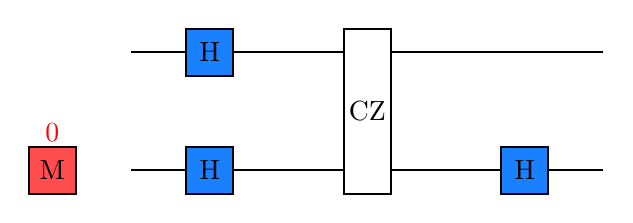
\begin{tikzpicture}[xscale=2]
\draw[string] (0.5,0) to +(3,0);
\draw[string] (0.5,1.5) to + (3,0);
\node[H] at (1,0) {H};
\node[H] at (1,1.5) {H};
\node[H] at (3,0){H};
%\path (0,1.5) node [M] {M} node [result] {0};
\path (0,0) node [M] {M} node [result] {0};
\node[CZ={1.5}] at (2,0.75) {CZ};
\end{tikzpicture}
\]

\vspace{20pt} Your qubits are now entangled - measuring one of them will yield the same result as measuring the other one.

%Make clear that if you do anything with the qubits after you've measured them, the entanglement is broken.

\end{frame}
}


\begin{frame}

\frametitle{SENDING INFORMATION}

%NEED A PICTURE. SAY: ``QUANTUM COMPUTERS WILL NEED TO TRANSFER ORDINARY BITS''

%\frametitle{SENDING NUMBERS}


Imagine you wanted to send your friend a ``0'' or a ``1''.

\vspace{7pt}
\textit{Could you do this using a qubit?}

\vspace{20pt}
Yes! Just press \inlineH then \inlineM until you get the number you want.

\vspace{7pt}
Then pass the qubit to your friend.

\vspace{7pt}
They can press \inlineM to discover the message.

\vspace{7pt}
\textbf{Let's try it!}

\vspace{20pt}
Could you send your friend \emph{two numbers} by passing them one qubit?

\end{frame}



\begin{frame}
\frametitle{SENDING INFORMATION}

\def\gap{10pt}

\textbf{Let's try it!} Get into pairs called Alice and Bob.

\vgap
\step 1 Entangle your qubits

\vgap

\begin{minipage}[t]{0.5\textwidth}
\textit{Alice's program:}

\vgap
\step 2 Secretly choose a \textit{first number} and\\\textit{second number}, each either 0 or~1

\vgap
\step 3 Press \inlineZ if your first number is~1

\vgap
\step 4 Press \inlineH

\vgap
\step 5 Press \inlineZ if your second number is~1

\vgap
\step 6 Give your qubit to Bob

\end{minipage}
\begin{minipage}[t]{0.471\textwidth}
\textit{Bob's program:}

\vgap
\step 7 Do \inlineCZ on both qubits

\vgap
\step 8 Press \inlineH separately on both qubits

\vgap
\step 9 Measure your original qubit.\\This gives Alice's \textit{first number!}

\vgap
\step {10} Measure Alice's qubit.\\This gives Alice's \textit{second number!}
\end{minipage}

\end{frame}

\begin{frame}
\frametitle{SENDING INFORMATION}

\def\gap{7pt}

\begin{minipage}{0.59\textwidth}
\raggedright

It seems like sending a qubit should transmit a \mbox{\textit{single number}.\hspace{-5cm}}

\vgap
But using entanglement, it can transmit \mbox{\textit{two numbers}.\hspace{-5cm}}

\vgap
\textit{How is this possible?}

\vgap
This picture represents our quantum program.

\vgap
One number gets transmitted when Alice passes her qubit to Bob.

\vgap
Some scientists have suggested the other number travels \textit{back in time}, through the entangled state.

\vgap
Probably not true. But it shows the difficult time scientists have understanding quantum computing.

\end{minipage}
\begin{minipage}{0.39\textwidth}
\[
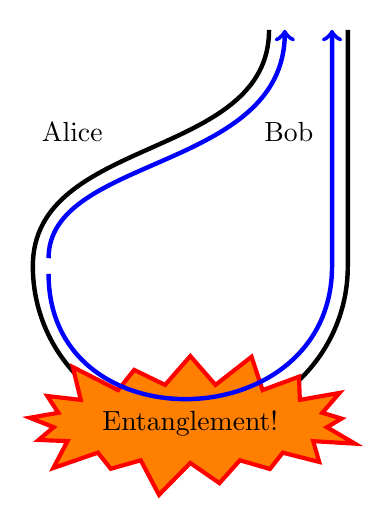
\begin{tikzpicture}
\draw [ultra thick] (0,0) to [out=left, in=down] (-2,2) to [out=up, in=down] (1,5);
\draw [ultra thick] (0,0) to [out=right, in=down] (2,2) to (2,5);
\node[starburst, draw, minimum width=3cm, minimum height=2cm, red, fill=orange, line width=1.5pt, text=black]
{Entanglement!};
\node at (-1.5,3.7) {Alice};
\node at (1.25,3.7) {Bob};
\draw [blue, ultra thick, ->] (-1.8,2.1) to [out=up, in=down, out looseness=0.8, in looseness=1.1] (1.2,5);
\draw [blue, ultra thick, ->] (-1.8,1.9) to [out=down, in=down, looseness=1.55] (1.8,2) to (1.8,5);
\end{tikzpicture}
\]
\end{minipage}

\end{frame}



\tikzset{top note/.style={align=center, above=0.35cm, font=\it}}

\ignore{
\begin{frame}
\frametitle{SENDING NUMBERS}
\begin{columns}[t]
\column{0.45\textwidth}{%
With entanglement, you can use \textit{one} qubit to send \textit{two} numbers.\\
 Get into pairs. Choose who will be the sender and receiver.

}
\column{0.5\textwidth}{%
The sender secretly chooses a first number (0 or 1), and a second number (0 or 1).


}
\end{columns}


\[
\def\scl{0.8}
\begin{tikzpicture}[scale=\scl, rotate=-90, every node/.style={rotate=0}]
\def\xgap{2.8}
\draw [string] (0,-0.5) to (0,5) to [out=up, in=down, looseness=0.5] node [align=center, sloped, font=\it] {give qubit to\\[-2pt]your friend} (\xgap-1,7) to +(0,3.5);
\draw [string] (\xgap,-0.5) to (\xgap,10.5);
\node [Z] at (0,0.5) {Z};
\node [top note] at (0,4.5) {only if second\\[-1pt]number is 1};
\node [H] at (0,2.5) {H};
\node [Z] at (0,4.5) {Z};
\node [top note] at (0,0.5) {only if first\\[-1pt]number is 1};
\draw [string, dashed] (0,-0.5) to +(0,-0.75);
\draw [string, dashed] (\xgap,-0.5) to +(0,-0.75);
\node [align=center, font=\it] at (0.5*\xgap,-0.9) {start with a pair of\\[-1pt]entangled qubits};
\node [CZ ={\scl}] at (\xgap-0.5,7.5) {CZ};
\node [H] at (\xgap,9.) {H};
\node [H] at (\xgap-1,9) {H};
\node [M] at (\xgap,10.5) {M};
\node [M] at (\xgap-1,10.5) {M};
\draw[dashed,->] (\xgap-1, 11.2) to +(0,0.5);
\draw[dashed,->] (\xgap, 11.2) to +(0,0.5);
\node[align=center, font=\it, right=0.01cm] at (\xgap-1, 11.7) {2nd number};
\node[align=center, font=\it, right=0.01cm] at (\xgap, 11.7) {1st number};
\end{tikzpicture}
\]
\vspace{-1cm}

\end{frame}
}

\begin{frame}
\frametitle{TELEPORTATION}

\splitpage{0.45}{
Quantum computers will need to move qubits around inside them.

\vgap
\uncover<2->{One of the most powerful ways to do this is called \textit{teleportation}.}
}
{
\[\begin{aligned}\begin{tikzpicture}
\node at (0,0) {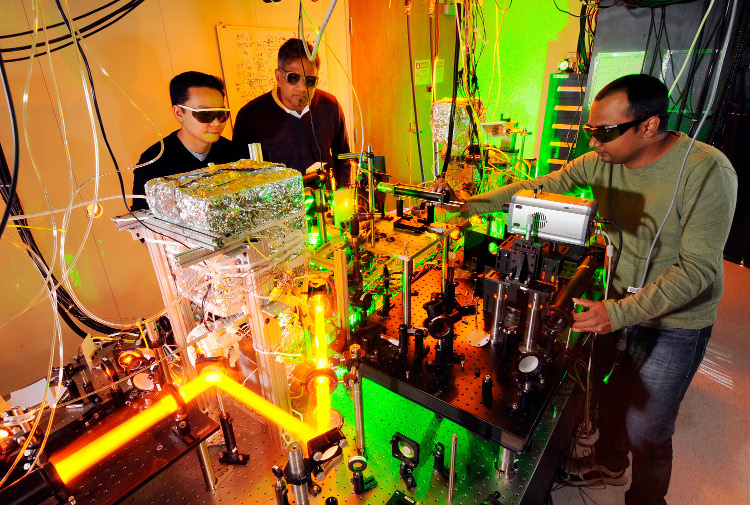
\includegraphics[height=3cm]{images/photoniccomputer}};
\end{tikzpicture}\end{aligned}\]
}

\splitpage{0.45}{
\uncover<3->{This uses \textit{entanglement} to move a qubit from one place to another.}

\vgap
\uncover<4->{It's not really what you're thinking of...}

\uncover<4->{but in the future, who knows?}
}{
\[\begin{aligned}\begin{tikzpicture}
\uncover<4->{\node at (0,0) {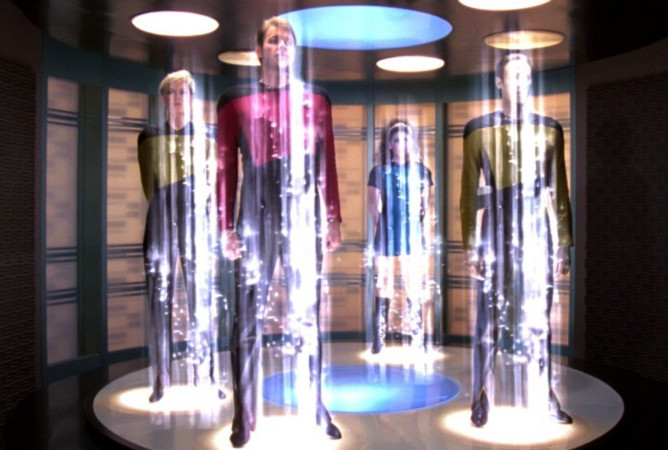
\includegraphics[height=3cm]{images/teleportation}};}
\end{tikzpicture}\end{aligned}\]
}

\end{frame}

\begin{frame}
\frametitle{TELEPORTATION}

\vspace{10pt}
\textbf{Let's try it!} Get into threes called Alice, Bob and Charlie.

\vspace{10pt}\pause
\step 1 Alice and Bob, entangle your qubits!

\vspace{10pt}\pause
\step 2 Charlie, press random buttons, then press \inlineM to get your \textit{secret number}.

\vspace{10pt}\pause
\step 3 Bob and Charlie, connect a cable, and both press \inlineCZ.

\vspace{10pt}\pause
\step 4 Bob, press \inlineH then \inlineM. If the answer is 1, then Alice press \inlineZ.

\vspace{10pt}\pause
\step 5 Alice, press \inlineH.

\vgap\pause
{\bf Charlie's qubit has now been teleported to Alice!}

%\vspace{10pt} \textit{Step 6.} Alice, press \inlineH then \inlineM. If the answer is 1, then Charlie press \inlineZ.

\vspace{10pt}\pause
\step 6 Alice, press \inlineM to discover {Charlie's secret number.}

\end{frame}

\ignore{
\begin{frame}
\frametitle{TELEPORTATION}

\textit{Step 3.} Alice and Bob, connect a cable, and both press \inlineCZ.

\vspace{15pt}
\textit{Step 4.} Bob, press \inlineH then \inlineM. If the answer is 1, then Charlie press \inlineZ.

\vspace{15pt}
\textit{Step 5.} Charlie, press \inlineH.

\vspace{15pt}
\textit{Step 6.} Alice, press \inlineH then \inlineM. If the answer is 1, then Charlie press \inlineZ.

\vspace{15pt}
\textit{Step 7.} Charlie, press \inlineM to get \textit{Alice's secret number!}

\end{frame}
}

\ignore{
\begin{frame}

\frametitle{TELEPORTATION}

\[
\begin{tikzpicture}[xscale=4]
\node at (0,-0.5) {\bf Alice};
\node at (1,-0.5) {\bf Bob};
\node at (2,-0.5) {\bf Charlie};
\node at (0,-2.5) {\inlineH};
\node at (1,-2.5) {\inlineH};
\draw [cable] (0,-1.5) node [miniCZ] {CZ} to +(1,0) node [miniCZ] {CZ};
\node at (-0.75,-1.5) {\it Step 4.};
\node at (-0.75,-2.5) {\it Step 5.};
\node at (-0.75,-3.5) {\it Step 6.};
\node [align=center] at (0,-3.5) {Press \inlineM to get\\\textit{Alice's number}};
\node [align=center] at (1,-3.5) {Press \inlineM to get\\\textit{Bob's number}};
\node at (-0.75,-4.5) {\it Step 7.};
\node [align=center] at (2,-4.5) {Press \inlineZ if\\Alice's number was 1};
\node at (-0.75,-5.5) {\it Step 8.};
\node at (-0.75,-6.5) {\it Step 9.};
\end{tikzpicture}
\]

\end{frame}
}

\ignore{
\begin{frame}
\frametitle{TELEPORTATION}

Get into pairs and entangle your qubits. \\
??
\tikzset{bottom note/.style={align=center, below=0.35cm, font=\it}}
\[
\begin{tikzpicture}
\def\ygap{2.5}
\draw[string] (-2,0) to +(5,0);
\draw[string] (-1,-1) to + (4,0);
\draw[string,dashed] (-2,-1) to +(1,0);
\draw[string,dashed] (-2,-1-\ygap) to +(1,0);
\draw[string] (-1,-1-\ygap) to + (10,0);
\node[CZ={1}] at (0.,-0.5) {CZ};
\node[H] at (1.5,-1) {H};
\node[H] at (1.5,0) {H};
\node[M] at (3,0) {M};
\node[M] at (3,-1) {M};
\node[Z] at (5,-1-\ygap) {Z};
\node[H] at (6.5,-1-\ygap) {H};
\node[Z] at (8,-1-\ygap) {Z};
\draw[dashed,->] (3.6,-1) to [out = right, in=up, looseness=0.9] (5,-0.4-\ygap);
\draw[dashed,->] (3.6,0) to [out = right, in=up, looseness=1.2] (8,-0.4-\ygap);
\node [align=center, font=\it] at (-1.5,-1-0.5*\ygap) {start with a pair of\\[-1pt]entangled qubits};
\draw[dashed, ->] (-3,0) to (-2.5,0);
\node[align=center, font=\it] at (-4,0) {your qubit};
\node[align=center,font=\it,rotate=20] at (6, -1-0.2*\ygap) {tell your friend your \\[-2pt] measurement outcomes};

\node [bottom note] at (5,-1-\ygap) {only if this\\[-1pt]outcome was 1};
\node [bottom note] at (8,-1-\ygap) {only if this\\[-1pt]outcome was 1};
\end{tikzpicture}
\]

\end{frame}
}

\ignore{
\begin{frame}
\frametitle{GHZ?}

\[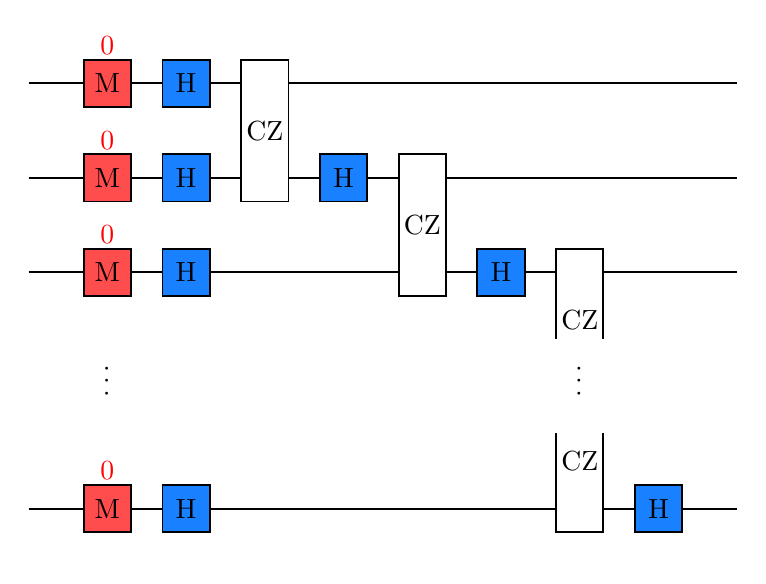
\begin{tikzpicture}
\def\ygap{1.2}
\draw[string] (0,0) to +(9,0);
\draw[string] (0,-\ygap) to + (9,0);
\draw[string] (0,-2*\ygap) to +(9,0);
\node[rotate=90] at (1,-3.15*\ygap){$\cdots$};
\draw[string] (0,-4.5*\ygap) to +(9,0);
\path (1,0) node [M] {M} node [result] {0};
\path (1,-\ygap) node [M] {M} node [result] {0};
\path (1,-2*\ygap) node [M] {M} node [result] {0};
\path (1,-4.5*\ygap) node [M] {M} node [result] {0};
\node[H] at (2,0) {H};
\node[H] at (2,-\ygap) {H};
\node[H] at (2,-2*\ygap) {H};
\node[H] at (2,-4.5*\ygap) {H};
\node[CZ={\ygap}] at (3, -0.5*\ygap) {CZ};
\node[H] at (4, -\ygap) {H};
\node[CZ={\ygap}] at (5,-1.5*\ygap) {CZ};
\node[H] at (6, -2*\ygap) {H};
\begin{scope}
\clip (0,0) rectangle (8, -2.7*\ygap);
\node[CZ={\ygap}] at (7,-2.5*\ygap) {CZ};
\end{scope}
\node[rotate=90] at (7,-3.15*\ygap){$\cdots$};
\begin{scope}
\clip (0, -5*\ygap) rectangle (8, -3.7*\ygap);
\node[CZ ={\ygap}] at (7,-4*\ygap){CZ};
\end{scope}
\node[H] at (8, -4.5*\ygap) {H};

\end{tikzpicture}
\]
\end{frame}
}

\begin{frame}
\frametitle{REAL QUANTUM COMPUTERS}

Real quantum computers don't exist yet. \pause Here's a plan for one we're building in Oxford:

\vspace{-5pt}
\[
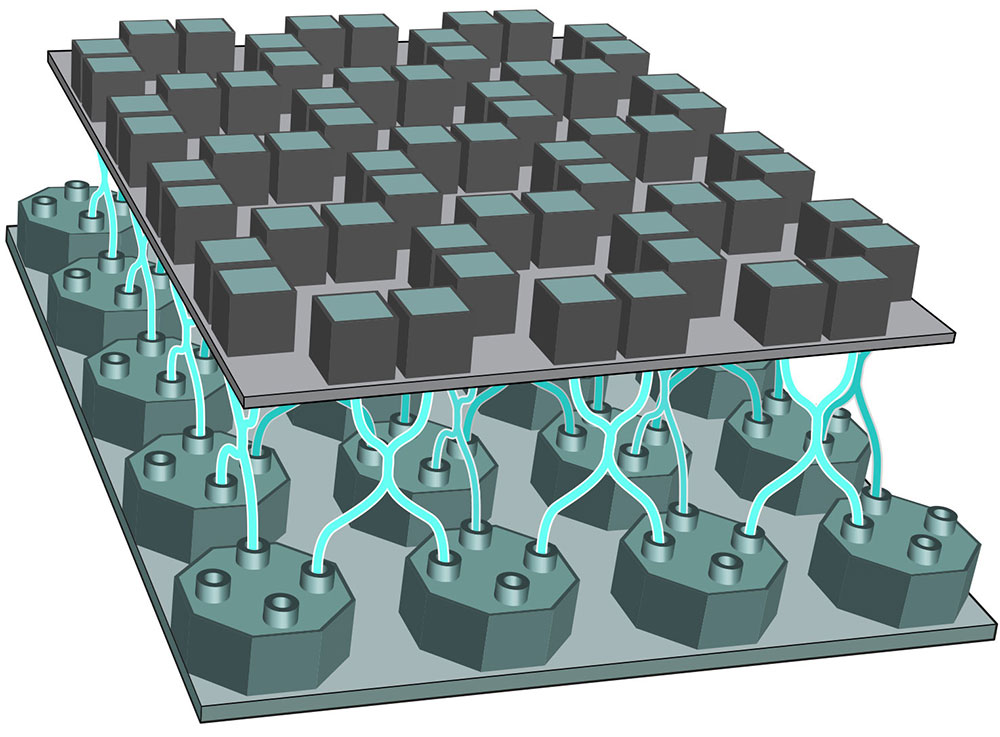
\includegraphics[height=4cm]{images/free/oxford_2020}
\]

\vspace{-5pt}\pause
Each of the little octagons will hold 20 qubits, giving the whole computer 400 qubits.

\vgap
We want to create entanglement and superposition across the \textit{whole computer}.

\vgap
It's hard because \textit{errors} can easily accumulate.

\end{frame}


\begin{frame}
\frametitle{REAL QUANTUM COMPUTERS}

\def\gap{7pt}
\textbf{Let's try it!} We'll do this challenge individually.

\vgap\pause
\textit{Step 1.} Everybody, store 0 in your qubit.

\vgap\pause
\textit{Step 2.} Everybody, press \inlineH.

\vgap\pause
\textit{Step 3.} Arrange your qubits in a single line, connected by cables.

\vgap\pause
\textit{Step 4.} First and second qubits press \inlineCZ, then the second qubit press \inlineH.

\vgap\pause
\textit{Step 5.} Second and third qubits press \inlineCZ, then the third qubit press \inlineH.

\vspace{0pt}
\hspace{2cm}\vdots

\vspace{3pt}\pause
\textit{Final Step.} Last two qubits press \inlineCZ, then last qubit press \inlineH.

\vgap\pause
{\bf Now everybody's qubits are entangled, and in superposition.}

\vgap\pause
Everybody, press \inlineM to measure your qubit!

\end{frame}



%{\usebackgroundtemplate{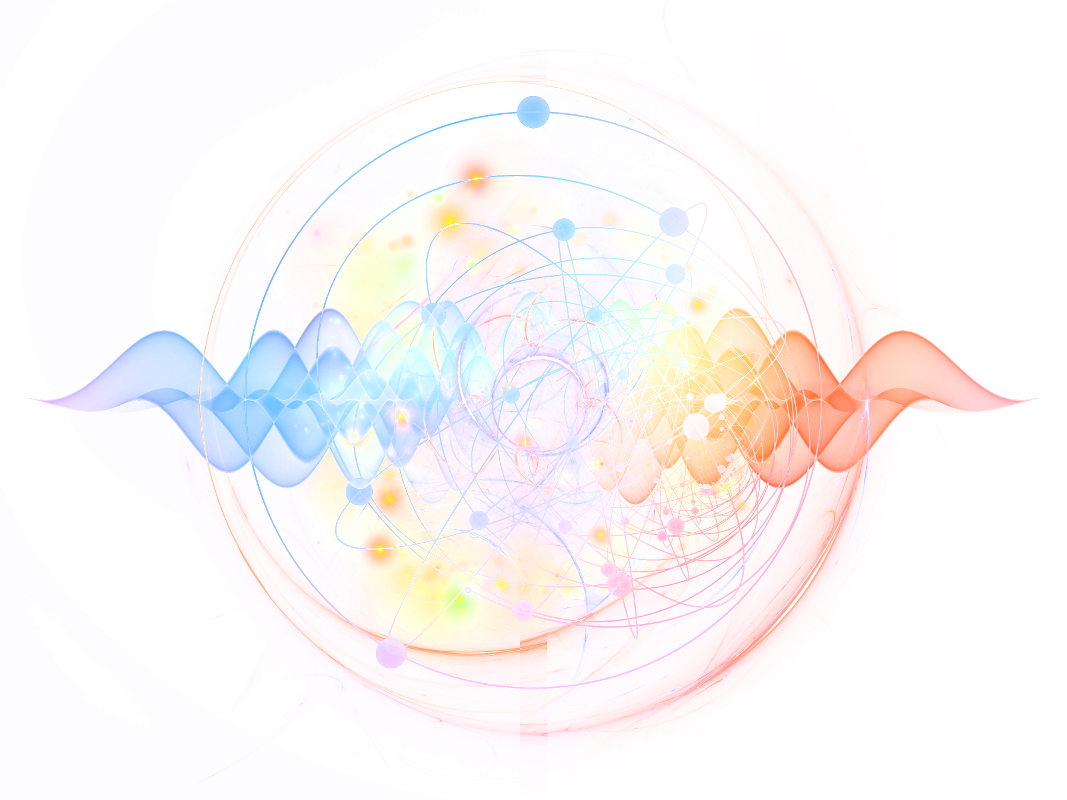
\includegraphics[width=\paperwidth]{paid/quantum_small_transparent}}%

\begin{frame}
\frametitle{THE END}
We've explored some amazing counter-intuitive features of reality which will drive technological advances over the next years.
\vspace{10pt}

\splitpage{0.5}{

\vspace{0.5cm}
\uncover<2->{In 2016, IBM launched the \textit{IBM quantum experience}, a 5 qubit quantum computer you can use over the internet. \uncover<3->{This month, IBM made an additional 16 qubit processor available.}}

\vspace{0.5cm}
\uncover<4->{Google is planning to build a 50 qubit quantum computer by the end of the year.}

\vspace{0.5cm}
\uncover<4->{}
}
{
\picturefamily{
\uncover<2->{\node [anchor=north west] at (0,0) {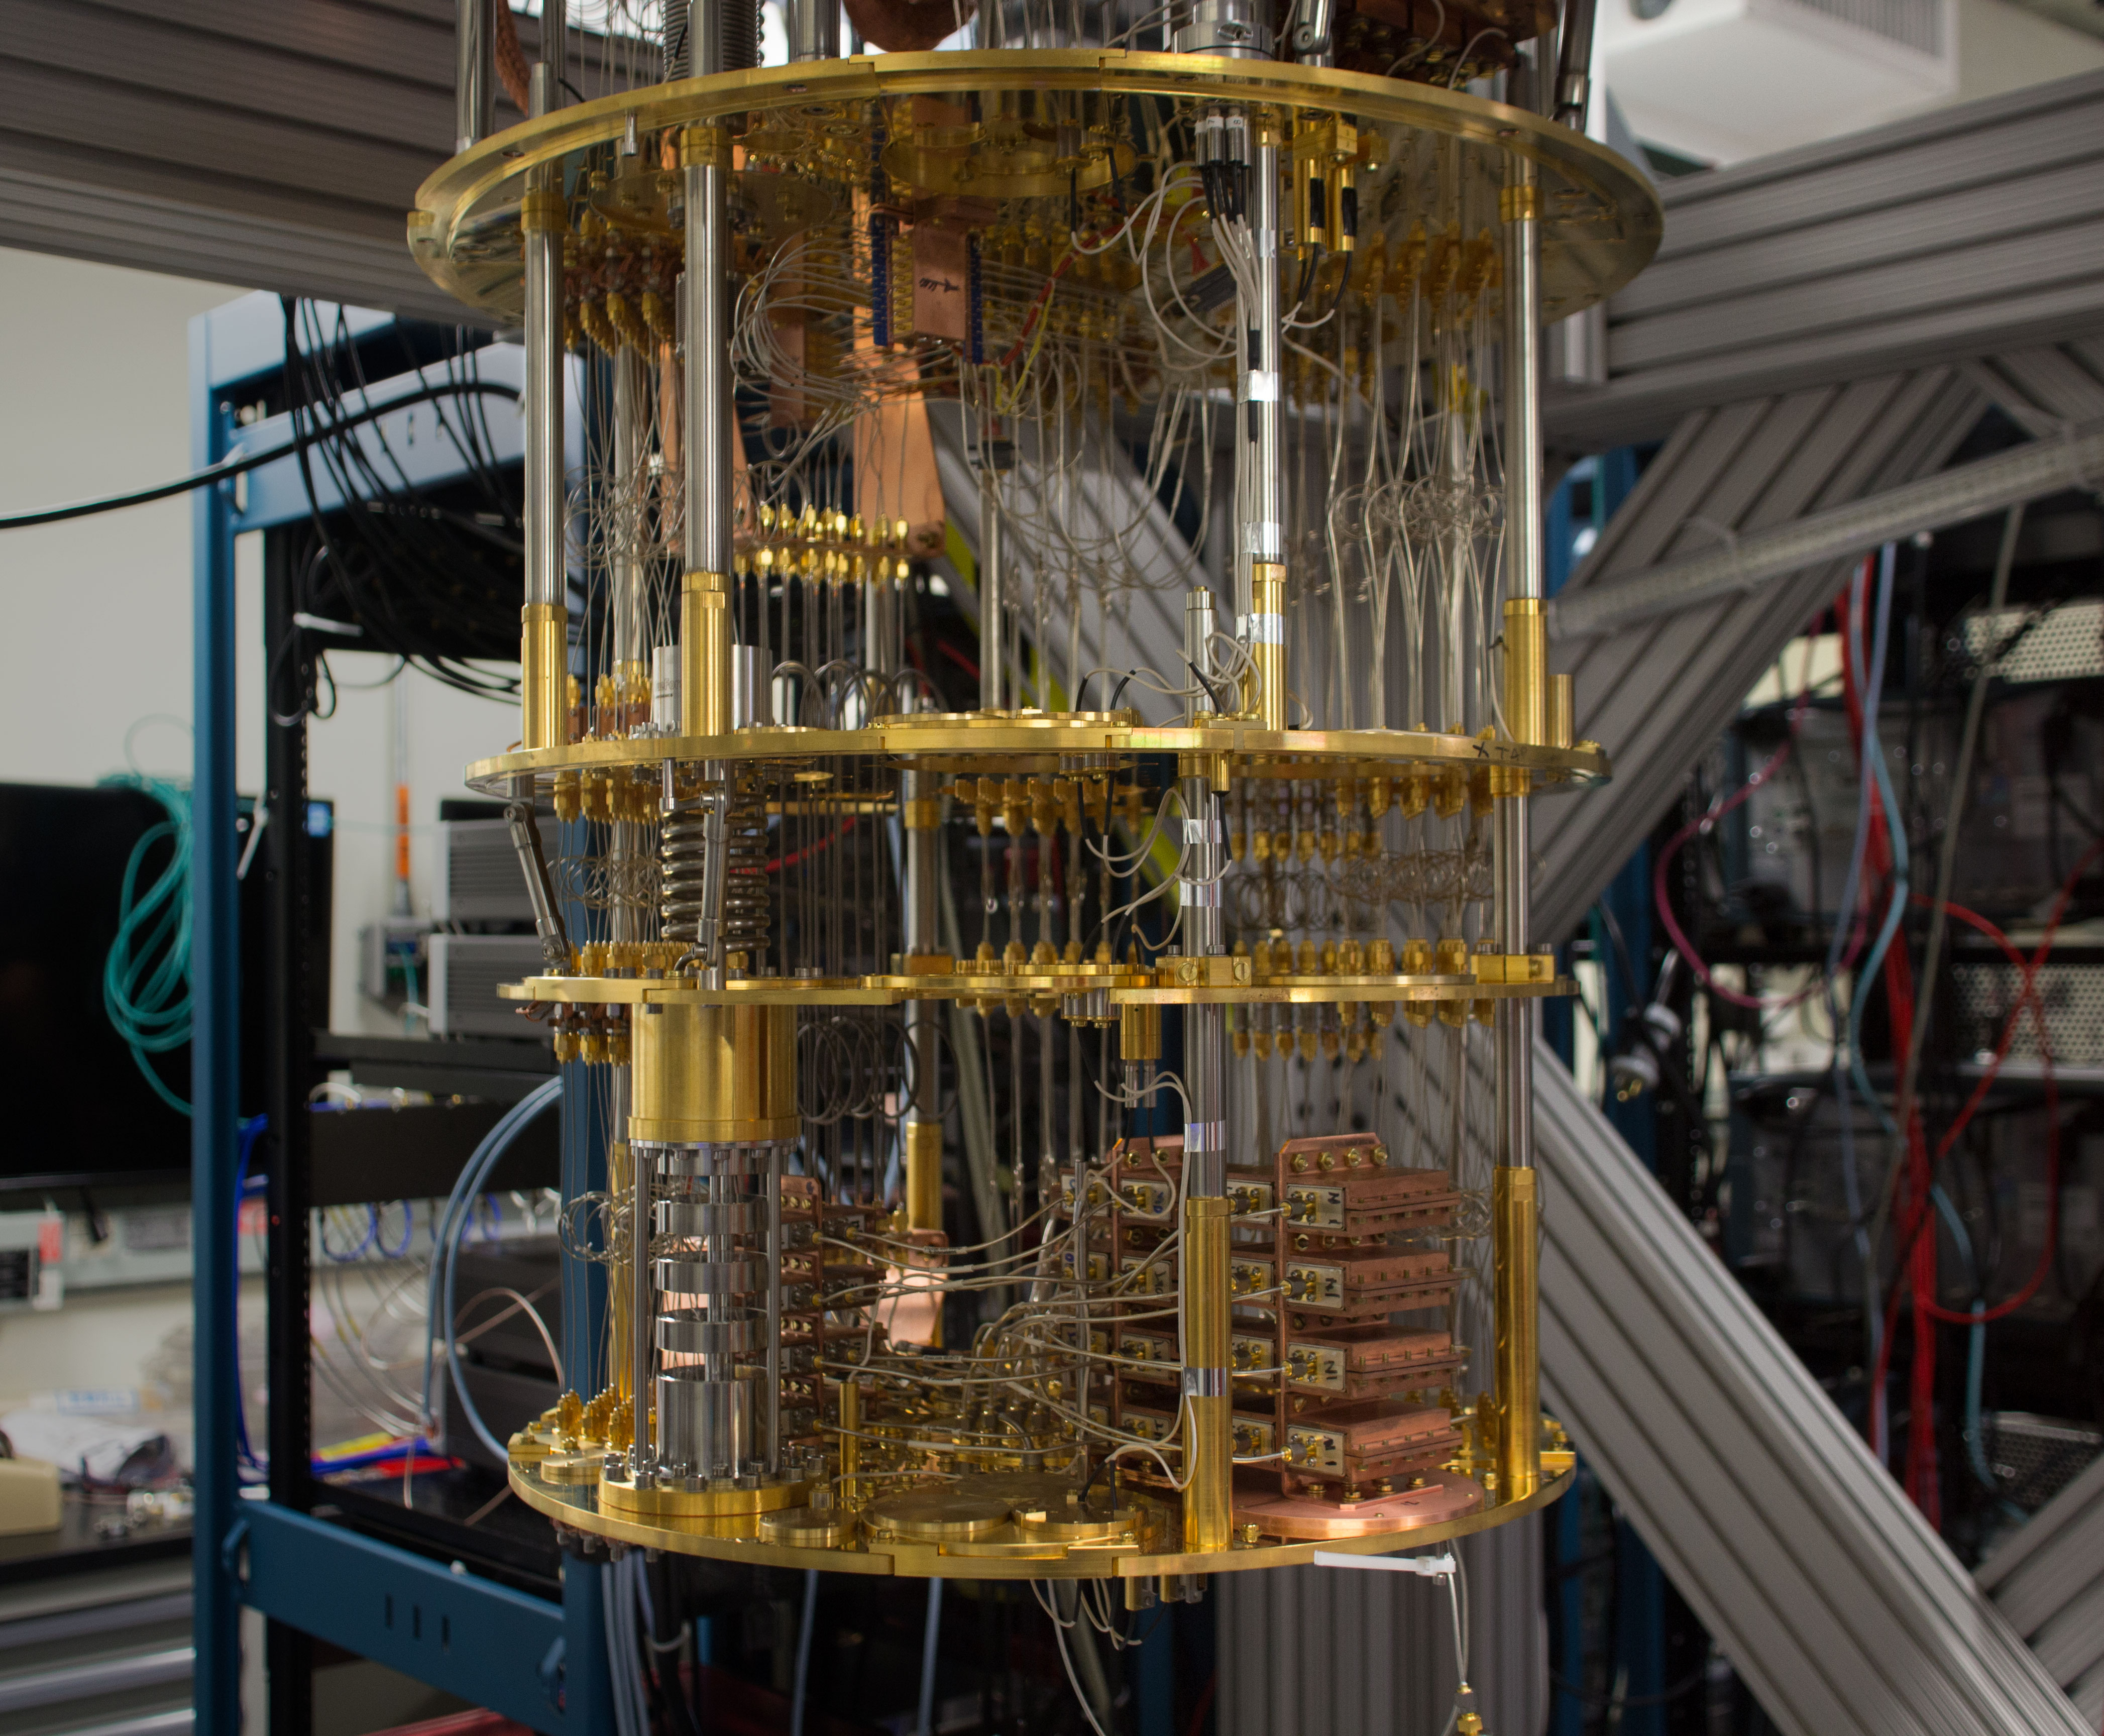
\includegraphics[width=5cm]{images/nonfree/IBM}};}
\uncover<4->{\node [anchor=north west] at (-0.5,-0.75) {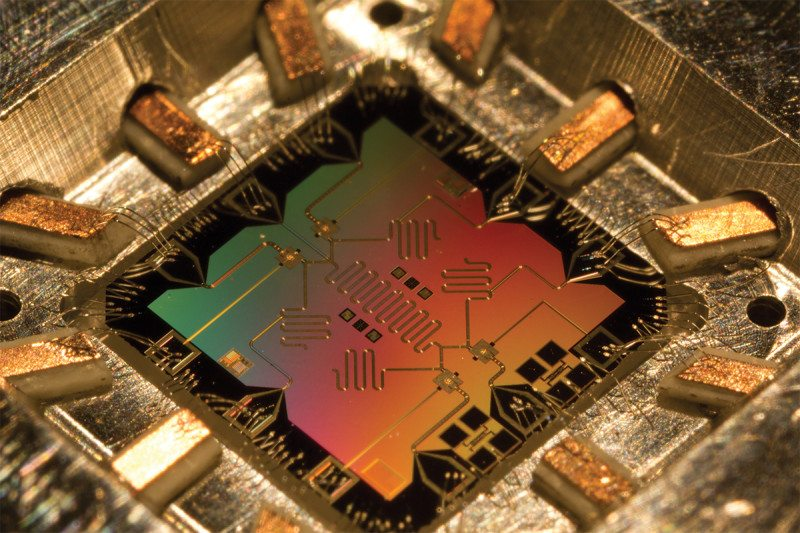
\includegraphics[height=3cm]{images/nonfree/UCSB}};}
}}

\vspace{25pt}
\centering
\uncover<5->{2017 is shaping up to be the year of the quantum computer.}



%\[
%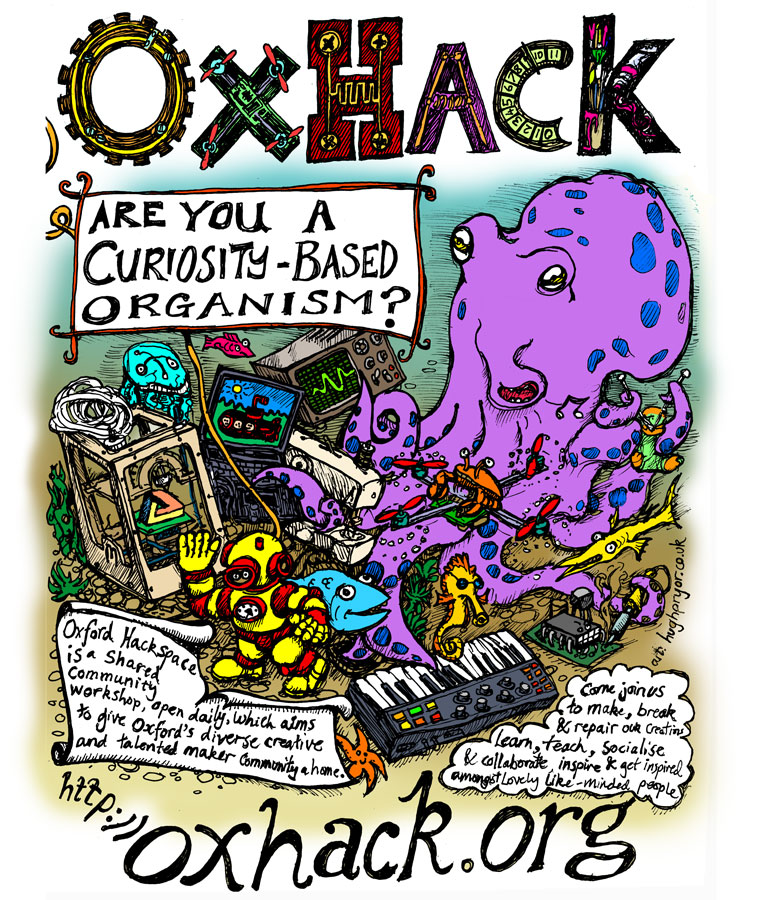
\includegraphics[height=6cm]{images/oxhack}
%\]


\end{frame}
%}




\end{document}\end{document}\end{document}

\begin{frame}
\section{Qubits}

\paragraph{What is a qubit?}

Scientists around the world are racing to build the first quantum computer, which will use the laws of quantum mechanics to solve some problems much faster than any computer we have now. Using your very own qubit, we can investigate some of the 

While today's computers store information using bits, quantum computers will store information using qubits

...

 - A qubit is the basic building block of a quantum computer
 
 - Measure, one-qubit operations, two-qubit operations
 
 - Using the cable
 
 - All the operations cancel themselves out if you do them twice. So if you press one by accident, press it again
 
 \section{Measurement}
 
You can ask a qubit the following question: ``what state are you in?''. The answer will be 0 or 1.

\section{Superposition}



\section{Entanglement}

Two entangled qubits will behave the same way, however far separated they are in space.

\paragraph{Experiment.} Entangle two qubits, then measure each of them.

\section{Teleportation}

\paragraph{Experiment.} 

\section{Super Dense Coding}

We can use qubits to send messages, by 

\end{frame}

\end{document}


\begin{frame}
\frametitle{Teleport entangled states.}
\vspace{5pt}
\tikzset{bottom note/.style={align=center, below=0.35cm, font=\it}}
\[
\begin{tikzpicture}
\def\ygap{2.5}
\draw[string] (-1,0.8*\ygap) to +(10,0);
\draw[dashed] (-2,0) to +(1,0);
\draw[dashed] (-2,0.8*\ygap) to +(1,0);
\node [align=center, font=\it] at (-1.5,0.5*0.8*\ygap) {start with a pair of\\[-1pt]entangled qubits};
\draw[string] (-1,0) to +(4,0);
\draw[string] (-1,-1) to + (4,0);
\draw[string,dashed] (-2,-1) to +(1,0);
\draw[string,dashed] (-2,-1-\ygap) to +(1,0);
\draw[string] (-1,-1-\ygap) to + (10,0);
\node[CZ={1}] at (0.,-0.5) {CZ};
\node[H] at (1.5,-1) {H};
\node[H] at (1.5,0) {H};
\node[M] at (3,0) {M};
\node[M] at (3,-1) {M};
\node[Z] at (5,-1-\ygap) {Z};
\node[H] at (6.5,-1-\ygap) {H};
\node[Z] at (8,-1-\ygap) {Z};
\draw[dashed,->] (3.6,-1) to [out = right, in=up, looseness=0.9] (5,-0.4-\ygap);
\draw[dashed,->] (3.6,0) to [out = right, in=up, looseness=1.2] (8,-0.4-\ygap);
\node [align=center, font=\it] at (-1.5,-1-0.5*\ygap) {start with a pair of\\[-1pt]entangled qubits};

\node[align=center,font=\it,rotate=20] at (6, -1-0.2*\ygap) {tell your friend your \\[-2pt] measurement outcomes};

\node [bottom note] at (5,-1-\ygap) {only if this\\[-1pt]outcome was 1};
\node [bottom note] at (8,-1-\ygap) {only if this\\[-1pt]outcome was 1};
\end{tikzpicture}
\]
\end{frame}
